\documentclass[a4paper,14pt]{article}
\usepackage{float}
\usepackage{extsizes}
\usepackage{amsmath}
\usepackage{amssymb}
\everymath{\displaystyle}
\usepackage{geometry}
\usepackage{fancyhdr}
\usepackage{multicol}
\usepackage{graphicx}
\usepackage[brazil]{babel}
\usepackage[shortlabels]{enumitem}
\usepackage{cancel}
\usepackage{textcomp}
\columnsep=2cm
\hoffset=0cm
\textwidth=8cm
\setlength{\columnseprule}{.1pt}
\setlength{\columnsep}{2cm}
\renewcommand{\headrulewidth}{0pt}
\geometry{top=1in, bottom=1in, left=0.7in, right=0.5in}

\pagestyle{fancy}
\fancyhf{}
\fancyfoot[C]{\thepage}

\begin{document}
	
	\noindent\textbf{6FMA49 - Matemática} 
	
	\begin{center}O tronco de pirâmide (Versão estudante)
	\end{center}
	
	\noindent\textbf{Nome:} \underline{\hspace{10cm}}
	\noindent\textbf{Data:} \underline{\hspace{4cm}}
	
	%\section*{Questões de Matemática}
	
	
    \begin{multicols}{2}
    	\noindent Obtemos um tronco de pirâmide ao "cortá-la" paralelamente à sua base.
    	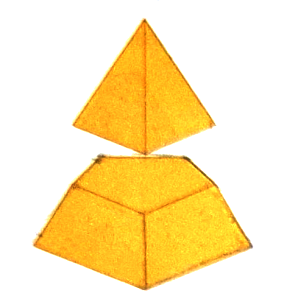
\includegraphics[width=1\linewidth]{imagens_6FMA49/imagem1}
    	No caso de uma pirâmide com base pentagonal, por exemplo, temos um tronco de pirâmide com 10 vértices, 7 faces e 15 arestas.
    	\noindent\textsubscript{~---------------------------------------------------------------------------}
		\begin{enumerate}
			\item Quantos vértices, quantas arestas e quantas faces tem o tronco de uma pirâmide de base hexagonal? Justifique. \\\\\\\\\\\\\\\\\\
			\item O monumento da foto é um obelisco, construído em Washington, capital dos Estados Unidos. Ele é composto por duas formas. Quais são elas? \\\\
			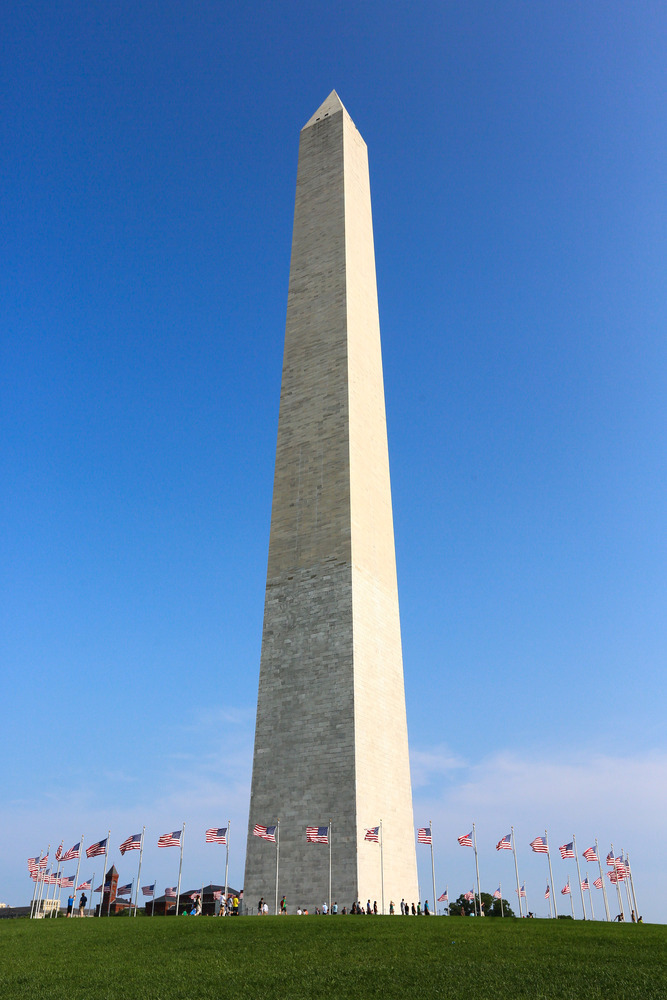
\includegraphics[width=1\linewidth]{imagens_6FMA49/washington-monument} \\\\\\\\\\\\\\\\\\\\\\
			\item Complete a tabela abaixo, colocando na coluna $V$ o número de vértices, na coluna $F$ o número de faces e na coluna $A$ o número de arestas. Na última coluna, coloque o valor da soma de $V$ com $F$ menos o valor de $A$. \\
			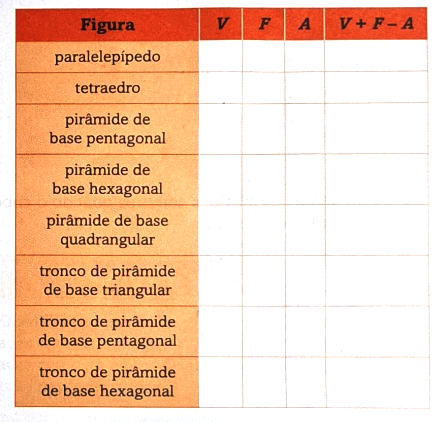
\includegraphics[width=1.1\linewidth]{imagens_6FMA49/imagem2}
			Procure interpretar os dados que aparecem na última coluna. Que conclusão você acredita que poderia tirar? \\\\\\\\\\\\\\\\
			\item Uma caixa tem o formato de um tronco de pirâmide de base pentagonal. Quantas faces e quantos vértices possui essa caixa? \\\\\\\\\\
			\item Um tronco de uma determinada pirâmide tem doze arestas. Que tipo de pirâmide é essa? \\\\\\\\\\\\\\\\
			\item Um tronco de uma determinada pirâmide tem 14 vértices. Quantas arestas possui a pirâmide que deu origem a esse tronco? \\\\\\\\\\\\\\\\
			\item Um tronco de pirâmide tem dez faces.
			\begin{enumerate}[a)]
				\item Qual é o polígono da base desse tronco? \\\\\\\\\\
				\item Quantas arestas e quantos vértices possui o tronco em questão? \\\\\\
				\item A relação $V - A + F = 2$ é satisfeita? ($V, A$ e $F$ são, respectivamente, o número de vértices, arestas e faces do tronco.) \\\\\\\\\\
			\end{enumerate}
		    \item Um tronco de pirâmide possui 18 vértices.
		    \begin{enumerate}[a)]
		    	\item Que tipo de tronco é esse? \\\\\\\\\\
		    	\item Quantas faces e quantas arestas possui esse tronco? \\\\\\\\\\
		    	\item A relação $V - A + F = 2$ é satisfeita? ($V, A$ e $F$ são, respectivamente o número de vértices, arestas e faces do tronco.)
		    \end{enumerate}
        \end{enumerate}
    $~$ \\ $~$ \\ $~$ \\ $~$ \\ $~$ \\ $~$ \\ $~$ \\ $~$ \\ $~$ \\ $~$ \\ $~$ \\ $~$ \\ $~$ \\ $~$ \\ $~$ \\ $~$ \\ $~$ \\ $~$ \\ $~$ \\ $~$ \\ $~$ \\ $~$ \\ $~$ \\ $~$ \\ $~$ \\ $~$ \\ $~$ \\ $~$ \\ $~$ \\ $~$ \\ $~$ \\ $~$ \\ $~$ \\ $~$ \\ $~$ \\ $~$ \\ $~$ \\ $~$ \\ $~$ \\ $~$ \\ $~$ \\ $~$ \\ $~$ \\ $~$ \\ $~$ \\ $~$ \\ $~$ \\ $~$ \\ $~$ \\ $~$ \\ 
    \end{multicols}
\end{document}